
\fancyhead[C]{Section 15.7}
\fancyhead[R]{\daynineteen}

\section*{\centering Chapter 15.7: Cylindrical and Spherical Coordinates}
\textbf{I3: Change of Variables.} I can use polar, cylindrical, and spherical coordinates to transform double and triple integrals and can sketch regions based on given polar, cylindrical, and spherical iterated integrals. I can use general change of variables to transform double and triple integrals for easier calculation.  I can choose the most appropriate coordinate system to evaluate a specific integral.\\\\
During studio, focus on \textit{setting up} the integrals. However, don't forget to carry out the actual integration in your own time. Both the correct triple integral and correct final answer are given in the answers for this worksheet.
\subsection*{Mechanics}
\begin{enumerate}
    \item \question{
    Use spherical coordinates to verify that the volume of a sphere with radius $\rho$ is $\dfrac{4}{3}\pi \rho^3$.
    }
        {% answer here
        
        }
        {% solution here
        
        }
    	
	\item \question{Use cylindrical coordinates to compute $\displaystyle \int_{-1}^1 \int_0^{\sqrt{1-y^2}} \int_0^x (x^2+y^2) \ dz \ dx \ dy$}
        {% answer here
        
        }
        {% solution here
        
        }
    
    \item \question{Find the volume of the solid that lies within the sphere $x^2+y^2+z^2=4$, above the $xy$-plane, and below the cone $z=\sqrt{x^2+y^2}$.}
        {% answer here
        
        }
        {% solution here
        
        }
     \item \question{Find the volume of the region bounded above by the paraboloid $z=9-x^2-y^2$, below by the $xy$-plane, and lying \emph{outside} the cylinder $x^2+y^2=1$.}
        {% answer here
        
        }
        {% solution here
        
        }
        \item \question{Suppose $a \geq 0$. Find the volume of the region cut from the solid sphere $\rho \leq a$ by the half-planes $\theta=0$ and $\theta= \pi/6$ in the first octant.}
        {% answer here
        
        }
        {% solution here
        
        }
        \item \question{When might you prefer to use cylindrical coordinates over spherical ones? In other words, is there a particular type of symmetry whose presence/absence suggests that cylindrical coordinates may be more useful?}
        {% answer here
        
        }
        {% solution here
        
        }
\end{enumerate}
\subsection*{Applications}
\begin{enumerate}[resume]
	
	\item \question{Let $D$ be the right circular cylinder whose base is the circle $r=2\sin \theta$ in the $xy$-plane and whose top is the plane $z=4-y$. Recall that $r=2 \sin \theta$ describes a circle centered at $(0,1)$ with radius $1$ in the $xy$-plane. Using cylindrical coordinates,
	\begin{enumerate}
		\item find the volume of the region $D$.
		\item find the $\bar{x}$ component of the centroid of the region. \textit{[Hint: Use symmetry.]}
	\end{enumerate}}
        {% answer here
        
        }
        {% solution here
        
        }
    \item \question{A double-scoop ice cream cone can be modeled by the region bound by the three component surfaces 
    \begin{align*}
        \textrm{Cone: }&9x^2+9y^2 -z^2= 0\qquad &&\textrm{for }0\leq z\leq 6 \\
        \textrm{Scoop One: }&x^2+y^2+(z-8)^2=9  \qquad &&\textrm{for }6\leq z\leq 10\\
        \textrm{Scoop Two: }&x^2+y^2+(z-12)^2 = 9\qquad &&\textrm{for }10\leq z
    \end{align*}
    Compute the volume of the entire dessert (including what is inside the cone, presumably more ice cream). \textit{[Hint: Do not compute the volume of the scoops as they are presented. Translate each scoop down so they are centered at the origin.]}
    \begin{center}
		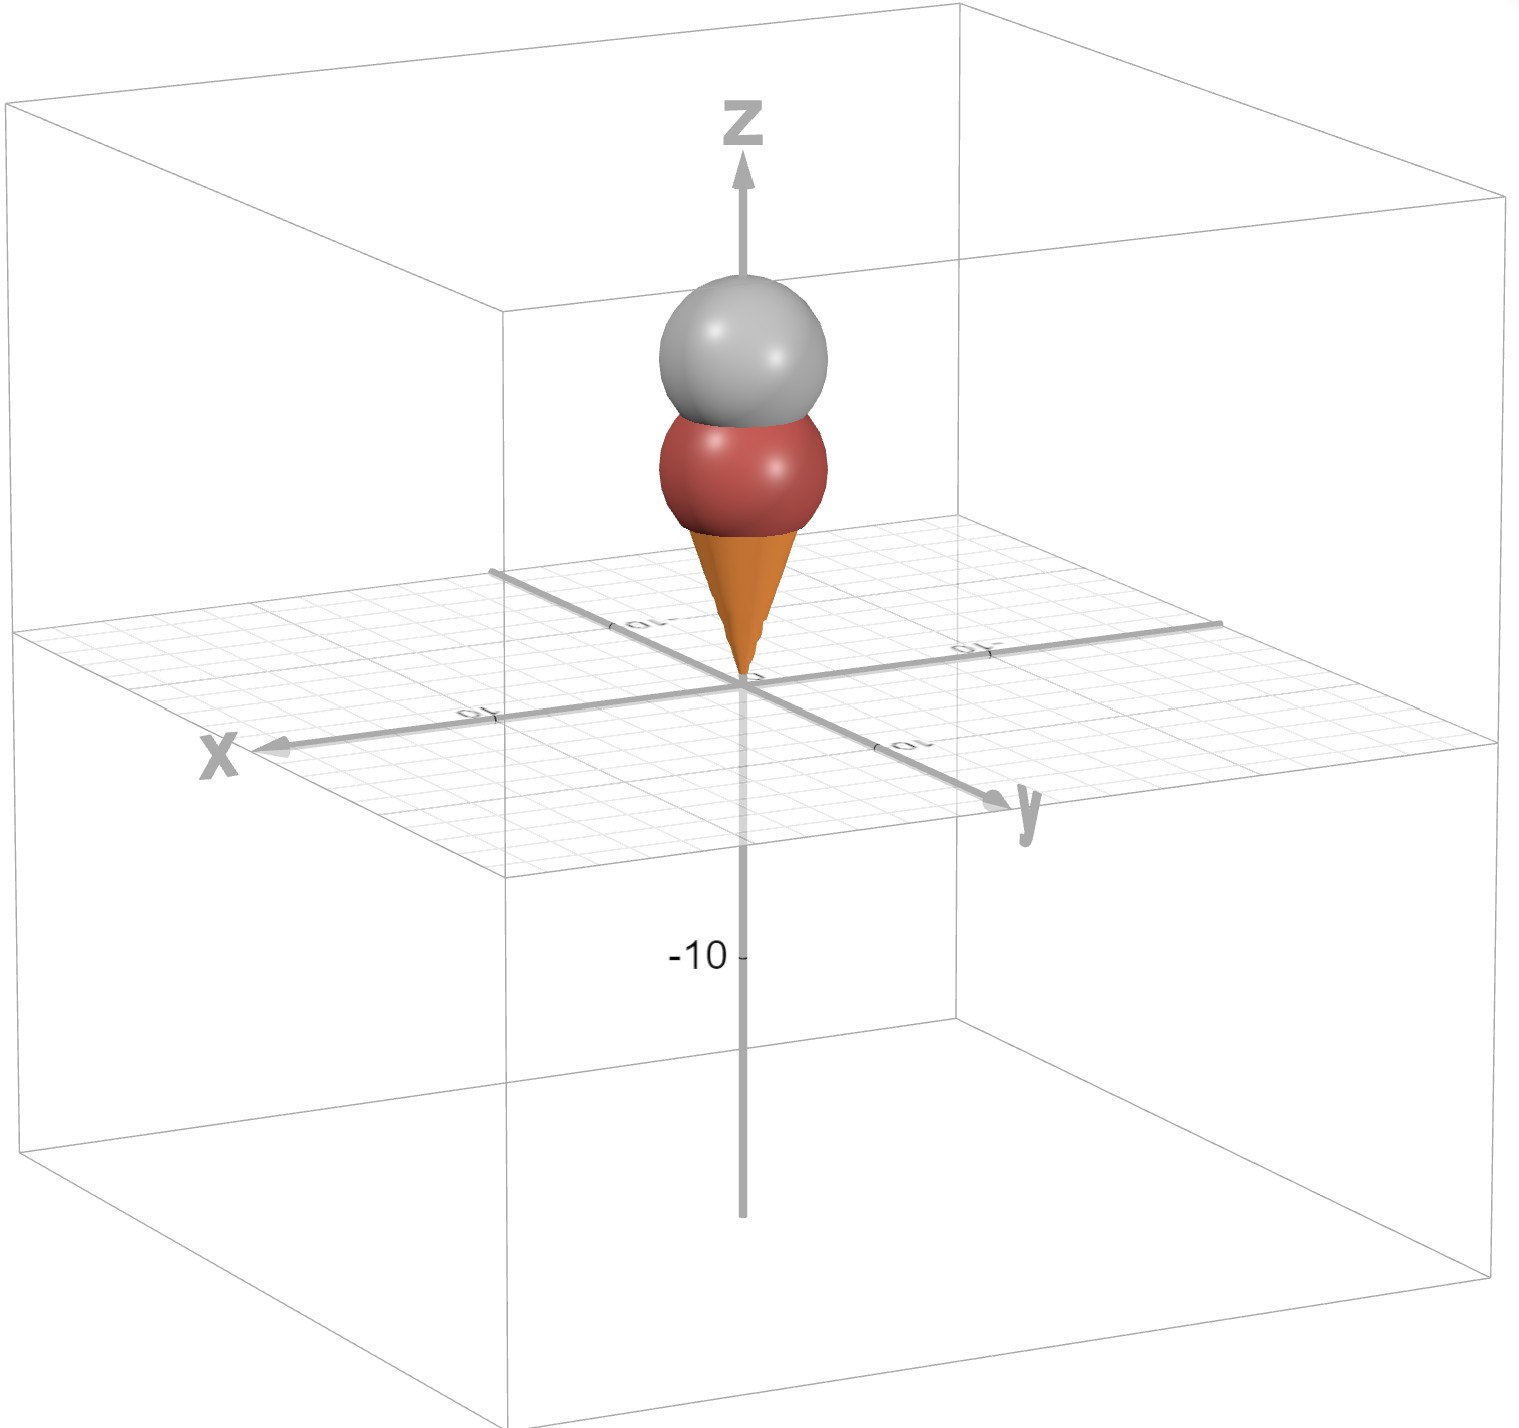
\includegraphics[scale=0.5,alt={ice cream cone and scoops}]{ice creammm.jpg}
	\end{center}}
        {% answer here
        
        }
        {% solution here
        
        }
\end{enumerate}
\subsection*{Extensions}
\begin{enumerate}[resume]
	\item \question{Let $B$ be the unit ball given by $x^2+y^2+z^2\leq 1$. Compute the average distance of a point in $B$ to the origin. Before you do any calculations, do you expect the average to be less than or greater than 0.5? Why? }
        {% answer here
        
        }
        {% solution here
        
        }
	
	\item \question{Find the volume of the solid that is between the spheres $\rho=\sqrt{2}$ and $\rho=2$, but outside of the circular cylinder $x^2+y^2=1$.  It will be helpful to draw a cross-section in a plane $\theta=c$ for this problem and to use symmetry.}
        {% answer here
        
        }
        {% solution here
        
        }

\end{enumerate}
{}

\iftoggle{answers}{
\begin{center}{\large \textbf{Math 2551 Worksheet Answers: Triple Integrals in Cylindrical \& Spherical Coordinates}}
\end{center}

\begin{enumerate}
	\item Integral: $\Ds \int_{-\pi/2}^{\pi/2} \int_0^1 \int_0^{r\cos(\theta)}r^3\ dz\ dr\ d\theta$
	
	Answer: $\dfrac{2}{5}.$
	
	\item Integral: $\Ds \int_0^{\pi/6} \int_0^{\pi/2} \int_0^a \rho^2\sin(\phi)\ d\rho\ d\phi\ d\theta$
	
	Answer: $\dfrac{a^3\pi}{18}.$
	
	\item Integral: $\Ds \int_0^{2\pi} \int_{\pi/4}^{\pi/2} \int_0^2 \rho^2\sin(\phi)\ d\rho\ d\phi\ d\theta$ 
	
	Answer: $\dfrac{8\sqrt{2}\pi}{3}$
	
	\item Integral: $\Ds \int_0^{2\pi} \int_1^3 \int_0^{9-r^2} r\ dz\ dr\ d\theta$
	
	Answer: $32\pi$
	
	\item Integral: $\Ds 2 \left( \int_0^{2\pi}\int_{\pi/6}^{\pi/4} \int_{\csc(\phi)}^{2} \rho^2\sin(\phi)\ d\rho\ d\phi\ d\theta +\int_0^{2\pi}\int_{\pi/4}^{\pi/2} \int_{\sqrt{2}}^{2} \rho^2\sin(\phi)\ d\rho\ d\phi\ d\theta \right)$
	
	Answer: $\dfrac{12\sqrt{3}-4}{3}\pi $.
	
	\item \begin{enumerate}
		\item Integral: $\Ds \int_0^{\pi} \int_0^{2\sin(\theta)} \int_0^{4-r\sin(\theta)} r\ dz\ dr\ d\theta$
		
		Answer: $3\pi.$
		\item $\bar{x}=0$.
	\end{enumerate}
\end{enumerate}

}{}
\iftoggle{solutions}
{
Solutions go here in the same format.
}{}
